\documentclass[a4paper]{article}
\usepackage{a4wide}
\usepackage{amsmath}
  \DeclareMathOperator*{\argmax}{arg\,max}
\usepackage{booktabs}
\usepackage{csquotes}
\usepackage{upquote}
\usepackage{float}
\usepackage{graphicx}
\usepackage{enumerate}
\usepackage{subcaption}
\usepackage{xcolor}
\usepackage{mcode}
\usepackage[numbered,framed]{matlab-prettifier}

\title{Pattern and Speech Recognition WS2015-16 \\ Exercise 3}
\author{Atanas Poibrenski(2554135), Marimuthu Kalimuthu(2557695), Furkat Kochkarov(2557017)}

\begin{document}

\maketitle
\section*{Dimensionality Reduction}

\section*{1 Preparation}
\subsection*{1.1 Loading and Plotting in the waveform}
\begin{enumerate}
	\item Linear classification - Iris dataset
	\begin{figure}[H]
		\begin{center}
			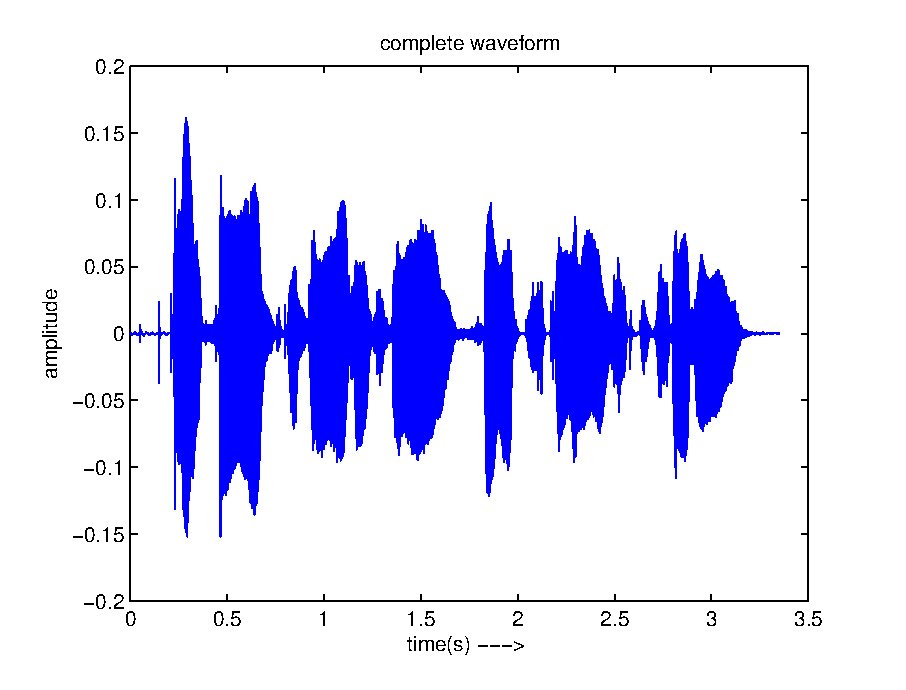
\includegraphics[width=0.85\textwidth]{ex2.eps}
			\caption{Complete waveform}\label{fig:comwavform}		
		\end{center}
	\end{figure}
	
	\item The dimensions of W must be n by 1.

\item Grid search

\end{enumerate}


%to include whole matlab file in the report
%\lstinputlisting{../code/ex02.m}
%\vspace{1em}


%to include a sample matlab code
%\begin{lstlisting}
% 	%return area of a triangle%
%	function [Area] = Area(a,b,c)
%	s = (a+b+c)/2;
%	Area = sqrt(s(s-a)*(s-b)*(s-c));
%	\end{lstlisting}



\end{document}
